% importa variabili globali
% definizione variabili globali
\def\GRUPPO {\textit{IDEA Studio web}}

\def\PROGETTO {\textbf{Biblioteca online}}

\def\PROGETTOESTESO {\textbf{Progetto per \textit{tecnologie web}}}

\def\COMMITTENTE {Prof.ssa Ombretta Gaggi}

\def\PROPONENTE {-}

\def\AZIENDA {IDEA Studio web}

\def\EMAIL {studioideaweb@gmail.com}

\def\LOGO {../template/img/logo.png}

\def\INTESTAZIONE {../template/img/intestazione.png}
\def\PIEDIPAGINA {../template/img/piedipagina.png}

\def\G {{\small $_G$}}



% definizione variabili locali
\def\DOCUMENTO{Relazione}
\def\VERSIONE{1.0.0}

\def\DESCRIZIONE{<Info documento>}

\def\REDATTORE {Francesco Bizzaro\\ & Gino Zaidan}
\def\VERIFICATORE {Luca Finotello\\ & Stefano Scaglione}
\def\RESPONSABILE {Bizzaro Francesco}

\def\USO {Interno}

\def\DISTRIBUZIONE {\GRUPPO{}\\ & \COMMITTENTE{}\\}

\def\DESCRIZIONE {Relazione del progetto \textit{\PROGETTO}, realizzato per il corso di \textit{tecnologie web} dal gruppo \GRUPPO}


% abilita (true) / disabilita (false) indice, lista tabelle, lista figure
\def\INDICE	{true}
\def\TABELLE {false}
\def\FIGURE {false}


% importa struttura
\input {../template/structure.tex}


% importa indici
\input {../template/index.tex}

% importa parti documento
\section{Organigramma}


Membri del gruppo \GRUPPO:
\begin{table}[h]
\centering
\bgroup
\def\arraystretch{1.6}
	\begin{tabular}{| c | c | c |}
		\hline 
		\rowcolor{LightCyan}
		\textbf{Nominativo} & \textbf{Matricola} & \textbf{Indirizzo di posta 
		elettronica} \\ \hline \hline 
		Francesco Bizzaro & 1069586 & francescob994@gmail.com  \\ \hline  
		Gino Zaidan & 1008249 & zaidan90@hotmail.it  \\ \hline 
		Luca Finotello & xxx & xxx  \\ \hline
		Stefano Scaglione & xxx & xxx  \\ \hline
	\end{tabular}
\egroup
\caption{Componenti}
\end{table}
\section{Scopo del progetto}
Si vuole realizzare il sito web di una biblioteca fittizia. In particolare, si vuole dare la possibilità agli utenti registrati di visualizzare il catalogo dei libri, effettuare ricerche, gestire i propri prestiti, e fare prenotazioni.\\
Per incentivare la lettura e lo scambio di opinioni, si vuole rendere \textit{social} il servizio, dando la possibilità ai lettori di pubblicare i propri commenti sui libri letti e consigliare libri ad altri utenti.



\textbf{[da ampliare..]}

\newpage
\section{Norme}
Il gruppo \GRUPPO\ ha deciso di imporsi delle regole per uniformare il lavoro e agevolare le fasi di sviluppo in team del sito web. Tali norme devono essere seguite da tutti i membri del gruppo. Il loro rispetto va controllato nelle fasi di verifica.

\subsection{Organizzazione}
\begin{itemize}
	\item Al termine di ogni sessione di lavoro, ogni file che ha subito modifiche deve essere validato nuovamente, o verificato da un membro del gruppo (non lo stesso che l'ha scritto)
	
	\item I membri del team devono utilizzare la casella di posta \EMAIL\ per ogni comunicazione ufficiale verso l'esterno
\end{itemize}

\subsection{Strumenti}
\begin{itemize}
	\item È stato creato un repository GitHub per contenere le pagine HTML, gli script perl, javascript e lo stile css. Alla fine di ogni sessione di lavoro i membri del team devono caricarvi i file creati o modificati (per semplificare il versionamento, evitare errori di sovrascrittura e minimizzare il rischio di perdita di dati)
\end{itemize}

\subsection{Codifica}
\begin{itemize}
	\item Ogni pagina html (anche se generata da script), ad eccezione della home, deve avere la stessa struttura di base decisa in fase di progettazione, con gli stessi tag (per creare consistenza)
	
	\item Tutti i tag o gli statement degli script devono essere indentati per garantire una maggiore leggibilità. Eventualmente, per risparmiare banda, le indentazioni possono essere tolte al termine della fase di sviluppo
	
	\item Gli script perl devono essere commentati. Le pagine HTML possono contenere dei commenti nelle prime versioni, ma questi devono essere tolti prima della consegna (per ragioni di efficienza)
	
	\item Tutti gli attributi id e class devono essere scritti secondo la sintassi XML, ossia senza spazi, con la prima lettera minuscola e la prima lettera di ogni parola successiva maiuscola (es. formRicerca). Non è permesso che un id inizi con un numero 
	
	\item I nomi dei file e delle cartelle non devono contenere spazi né caratteri speciali, ad eccezione del carattere di underscore (\_), da usare al posto dello spazio. Devono inoltre essere scritti completamente in minuscolo
	
\end{itemize}

\newpage
\section{Analisi dei requisiti}
[inserimento di alcuni scenarios per descrivere i casi d'uso principali..]
\section{Progettazione}
In relazione ai requisiti individuati nella sezione precedente, sono state progettate le interfacce che le pagine dovranno avere e la loro architettura ad alto livello.


\subsection{Home}
[descrizione home..]
\begin{figure}[H]
	\centering
	\includegraphics[width= 14cm]{immagini/home.png}
	\caption{Home page}
\end{figure}

\subsection{Catalogo}
[descrizione catalogo..]
\begin{figure}[H]
	\centering
	\includegraphics[width= 14cm]{immagini/catalogo.png}
	\caption{Catalogo dei libri}
\end{figure}

\subsection{Dettaglio}
\textbf{[descrizione dettagli]}
\begin{figure}[H]
	\centering
	\includegraphics[width= 14cm]{immagini/dettaglio.png}
	\caption{Visione di dettaglio dei libri}
\end{figure}

\subsection{Servizi}
[descrizione servizi..]
\begin{figure}[H]
	\centering
	\includegraphics[width= 14cm]{immagini/servizi.png}
	\caption{Servizi offerti e regolamento}
\end{figure}

\subsection{Contatti}
[descrizione contatti..]
\begin{figure}[H]
	\centering
	\includegraphics[width= 14cm]{immagini/contatti.png}
	\caption{Indicazioni e recapiti}
\end{figure}

\subsection{Prenotazione}
[descrizione prenotazione..]

\subsection{Gestione prestiti}
[descrizione gestione prestiti..]

\subsection{Profilo utente}
[descrizione profilo utente..]

\subsection{Amministrazione}
\subsubsection{Conferma account}
[descrizione conferma account..]

\subsubsection{Inserimento libro}
[descrizione inserimento libro..]

\subsubsection{Rimozione commento}
[descrizione rimozione commento..]



%\input {sections/nomesezione}
%\newpage

% ...

%\printglossaries

\end{document}
